\appendix
%% Правка оформления ссылок на приложения:
%http://tex.stackexchange.com/questions/56839/chaptername-is-used-even-for-appendix-chapters-in-toc
%http://tex.stackexchange.com/questions/59349/table-of-contents-with-chapter-and-appendix
%% требует двойной компиляции
\addtocontents{toc}{\def\protect\cftchappresnum{\appendixname{} }%
\setlength{\cftchapnumwidth}{\widthof{\cftchapfont\appendixname~Ш\cftchapaftersnum}}%
}
%% Оформление заголовков приложений ближе к ГОСТ:
\sectionformat{\chapter}[display]{% Параметры заголовков разделов в тексте
    label=\chaptertitlename\ \thechapter,% (ГОСТ Р 2.105, 4.3.6)
    labelsep=20pt,
}
\renewcommand\thechapter{\Asbuk{chapter}} % Чтобы приложения русскими буквами нумеровались

\chapter{Единицы измерения потока фотонов}
В области синхротронного излучения приняты специфические единицы измерения потока фотонов:
\begin{equation}
	\Phi = \cfrac{\gamma}{\textup{сек} \cdot 0.1\%\textup{bw} \cdot \textup{мм}^2}
\end{equation}
Для удобства была введена необычная единица $0.1\%\textup{bw}$, которая описывает энергетический диапазон, --- количество фотонов попавшее в полосу пропускания шириной $0.1\%$ на некоторой фиксированной энергии гамма-квантов, т.е., например, для энергии $1000 \;\textup{эВ}$ ширина полосы будет в диапазоне $999,5 - 1000,5 \; \textup{эВ}$. 
%Данная единица была введена, для удобства оценок потоков, после прохождения излучения через кристаллические монохроматоры и решёточные монохроматоры, полосы пропускания которых как раз составляют порядка $10^{-3} - 10^{-4}$. 

Иногда возникает потребность перевести эти единицы, например, к виду:
\begin{equation}
\Phi = \cfrac{\gamma}{\textup{сек} \cdot \textup{эВ} \cdot \textup{мм}^2}
\end{equation} 
Сделать это можно следующим образом, необходимо поточено умножить спектральное распределение на множитель $\cfrac{0.1 \% \cdot E_{\gamma}}{1\textup{эВ}}$, что даст необходимые единицы измерения. Далее, более тривиально, спектр можно привести к виду:
\begin{equation}
\Phi = \cfrac{W}{1\textup{эВ} \cdot \textup{мм}^2},
\end{equation} 
где $W$ --- мощность падающего излучения. В таких единицах, удобно, например, описывать тепловые нагрузки на оптические элементы.

\iffalse
\chapter{Учёт конечности эмиттанса}
В этом части мы покажем влияние эмиттанса электронного пучка на спектр излучения и угловое распределение. Для начала перепишем уравнение~\ref{eq:field_dist_Norm} с учётом отклонения частиц от заданной траектории, --- $h_x$ и $h_y$ и с некоторым дополнительным углом $\eta_x$ и $\eta_x$. Сразу можно понять, что в уравнении~\ref{eq:field_dist_Norm} можно сделать замену $\theta_{x,y} \rightarrow \theta_{x,y} - \eta_{x, y} - \cfrac{l_{x,y}}{z_0}$ и переписать углы в нормализованных единицах аналогично с~\ref{eq:norm_units}, с точностью до фазы: 
\begin{equation}
\label{eq:field_dist_Norm}
\begin{array}{lcl}
\hat{E}_{\bot} \sim
\sinc\bigg[\cfrac{\hat{C}}{2} + 
\cfrac{1}{4}\bigg(\hat{\theta}_{x} - \hat{\eta}_{x} - \cfrac{l_{x}}{z_0}\bigg)^2 +
\cfrac{1}{4}\bigg(\hat{\theta}_{y} - \hat{\eta}_{y} - \cfrac{l_{y}}{z_0}\bigg)^2\bigg],
\end{array}	
\end{equation}
При этом можно положить  $\cfrac{l_{x,y}}{z_0} \ll 1$, что выполняется с очень высокой точностью. 

В наших рассуждениях мы будем использовать предельный случай: электронный пучок не симметричен его вертикальный размер много меньше размера по радиальному направлению. Распределение частиц будем считать гауссовым: 
\begin{equation}
\label{eq:field_dist_Norm}
h_{x, y}(\eta_{x, y}) = \cfrac{N_e}{\sqrt{2\pi}\sigma_{x', y'}} \exp[-\cfrac{\eta^2_{x, y}}{2\sigma^2_{x', y'}}]
\end{equation}

Для удобства перепишем это распределение в нормализованных единицах, помня $\sigma_{x', y'} = \epsilon_{x', y'}/\beta_{x', y'}$, где $\epsilon_{x', y'}$ --- вертикальный и горизонтальный эмиттансы, $\beta_{0x', y'}$ --- бета-функция. Нормализованные единицы для $\hat{\beta}_{0} = L^{-1}_{\omega}\beta_{0}$
и $\hat{\epsilon} = (\omega/c)\epsilon$
\begin{equation}
\label{eq:field_dist_Norm}
h(\hat{\eta}) = \cfrac{1}{\sqrt{2\pi\hat{\epsilon}/\hat{\beta}}} \exp[-\cfrac{\hat{\eta}^2\hat{\beta}_{0}}{2\hat{\epsilon}^2}]
\end{equation}
Как уже упоминалось мы будем рассматривать предельный случай $\epsilon_{y'}/\beta_{y'} \ll 1$, в то время как $\hat{\beta_0}_{x,y} \sim 1$, поэтому просто $\epsilon_{y'} \ll 1$. Теперь можно записать интенсивность поля следующий образом: 
\begin{equation}
\label{eq:convolution}
\hat{I} = \cfrac{1}{\sqrt{2\pi\hat{\epsilon}/\hat{\beta}}}
\displaystyle\int\limits_{-\infty}^{\infty} d\hat{\eta}_x \sinc^2(\zeta)	
\exp[-\cfrac{\hat{\eta}_x^2\hat{\beta}_{0x}}{2\hat{\epsilon}_x}],д
\end{equation}
Где мы ввели $\zeta = \cfrac{\hat{C}}{2} + 
\cfrac{1}{4}(\hat{\theta}_{x} - \hat{\eta}_{x})^2 +
\cfrac{1}{4}\hat{\theta}_{y}^2$. Здесь мы учли, что распределение по $y$ действует как дельта-функция. Предыдущее уравнение упрощается дальше в пределе $\hat{\epsilon}_x\hat{\beta}_x \gg 1$, опять же помня, что и $\hat{\beta}_x \sim 1$, получается $\hat{\epsilon}_x \gg 1$. Ширина $\sinc^2(\zeta)$ много больше ширины гауссвоского распределения, ширина которого $\hat{\epsilon}_x$, поэтому интеграл будет набираться в пике кардинального синуса и экспоненту можно вынести с аргументом: $\hat{\eta}_x = \hat{\theta}_x$: 
\begin{equation}
\label{eq:convolution}
\hat{I} = \cfrac{\exp[-\hat{\theta}_x^2\hat{\beta}_{0x}/2\hat{\epsilon}_x]}{\sqrt{2\pi\hat{\epsilon}/\hat{\beta}}}
\displaystyle\int\limits_{-\infty}^{\infty} d\hat{\eta}_x \sinc^2\bigg(\cfrac{\hat{C}}{2} + 
\cfrac{1}{4}(\hat{\theta}_{x} - \hat{\eta}_{x})^2 +
\cfrac{1}{4}\hat{\theta}_{y}^2\bigg)	
\end{equation}
\begin{figure}[h!]
	\centering  
	\begin{minipage}{0.49\textwidth}
		\centering
		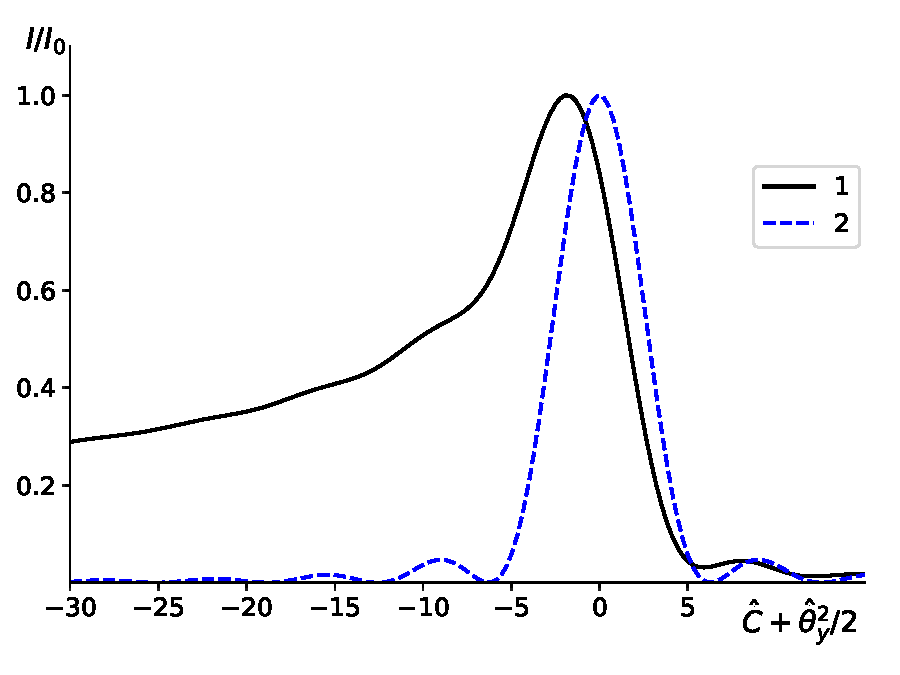
\includegraphics[width=\textwidth]{pic/spec_integ_emittance.pdf}
		\caption{Нормализованный спектр ондуляторного излучения. Линия 1 - спектр с учётом эмиттанса, линия 2 - спектр излучения уединённого электрона}
		\label{fig:2spec_emittance_and_single}
	\end{minipage}\hfill
	\begin{minipage}{0.49\textwidth}
		\centering
		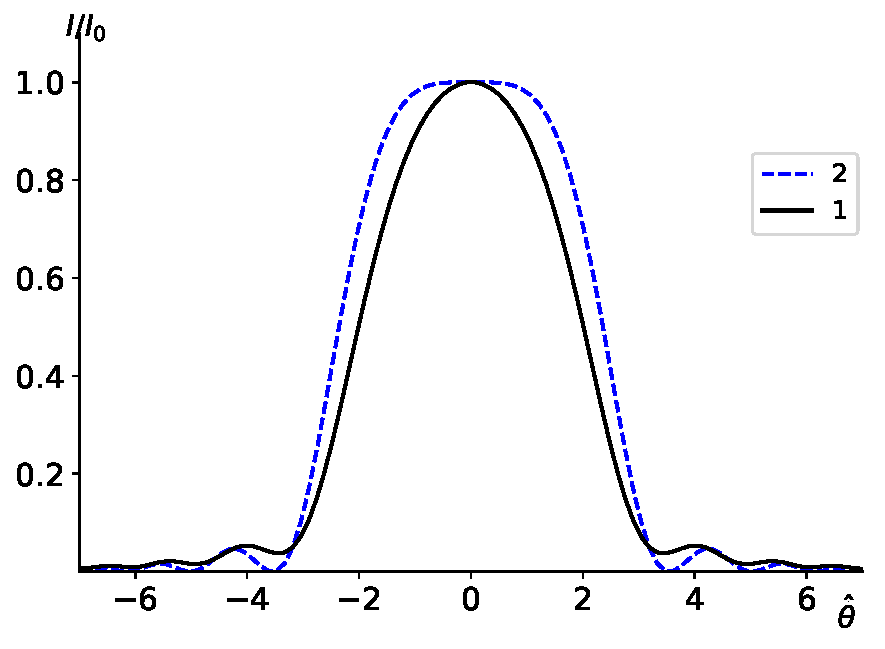
\includegraphics[width=\textwidth]{pic/angle_integ_emittance.pdf}
		\caption{Нормализованное угловое распределение излучения. Линия 1 - спектр с учётом эмиттанса, линия 2 - спектр излучения уединённого электрона}
		\label{fig:spec}
	\end{minipage}    
\end{figure}
Этот интеграл можно взять числено. %введя очевидную замену $\hat{\eta_{x}} \rightarrow \hat{\theta}_x - \hat{\eta_{x}}$. 
На~\ref{fig:2spec_emittance_and_single} представлены: линия 1.: спектр излучения пучка с $\hat{\epsilon}_x\rightarrow \infty$  $\hat{\epsilon}_y\rightarrow 0$, линия 2.: спектр одиночного электрона как функция $\hat{C} + \hat{\theta}_y^2/2$ при $\hat{\theta}_x = 0$, на рис.~\ref{fig:spec} то же для распределения интенсивности по углам. 

Итого, в этой главе мы привели один из случаев учёта конечности эмиттанса, который с хорошей точностью применим в современных источниках синхротронного излучения третьего и четвёртого поколений. В многом, данного подхода достаточно для того, чтобы интерпретировать резултаты вычислений кода SRW, при необходимости взятые нами приближения могут быть изменены и так же полученные результаты при помощи богатых вычислительных способностей современных ЭВМ.

\chapter{Состав высших гармоник ондуляторного излучения}
При рассмотрение излучения электрона в планарном ондуляторе мы не затрагивали вопрос, какие кратные гармоники присутствуют в спектре планарного ондулятора. Чтобы разобраться в этом вопросе надо принять учесть запаздывание по времени, в которое наблюдатель принял излучение, т.е. записывая известное соотношение $t = t' + \cfrac{1}{c} |R - r(t')|$, где за $t$ мы обозначили время наблюдателя, а $t'$ время излучателя. Дифференцированием этого выражения по $t'$ можно получить: $\cfrac{dt}{dt'} = 1 - \vec{n}\cdot\vec{\beta}$, где $\vec{\beta} = \vec{v}/c$. Подставляя решение для скорости~\ref{eq:eq_of_motion_velocity} и решая дифференциальное уравнение согласно \cite{als2011elements}, можно получить решение, которое даёт соотношение на время наблюдателя и время излучателя.
\begin{equation}
\label{eq:t_t'}
\omega t = \omega_w t' + \cfrac{K^2/4}{1 + (\gamma \theta)^2 + K^2/2} \sin(2 \omega_w t') - \cfrac{2K\gamma}{1 + (\gamma \theta)^2 + K^2/2} \; \phi \sin(\omega_w t') 	
\end{equation}
Здесь $\phi$ --- вертикальный угол наблюдения, а $\theta$ суммарный угол наблюдения --- $\theta = \sqrt{\phi^2 + \psi^2}$, где $\psi$ --- горизонтальный угол наблюдения. Из решения уравнения~\ref{eq:eq_of_motion_trej} знаем, что траектория, в общем, пропорциональна $\sin$, можно построить зависимость отклонения частицы от времени излучателя и наблюдателя:
\begin{figure}[h!]
	\centering  
	\begin{minipage}{0.46\textwidth}
		\centering
		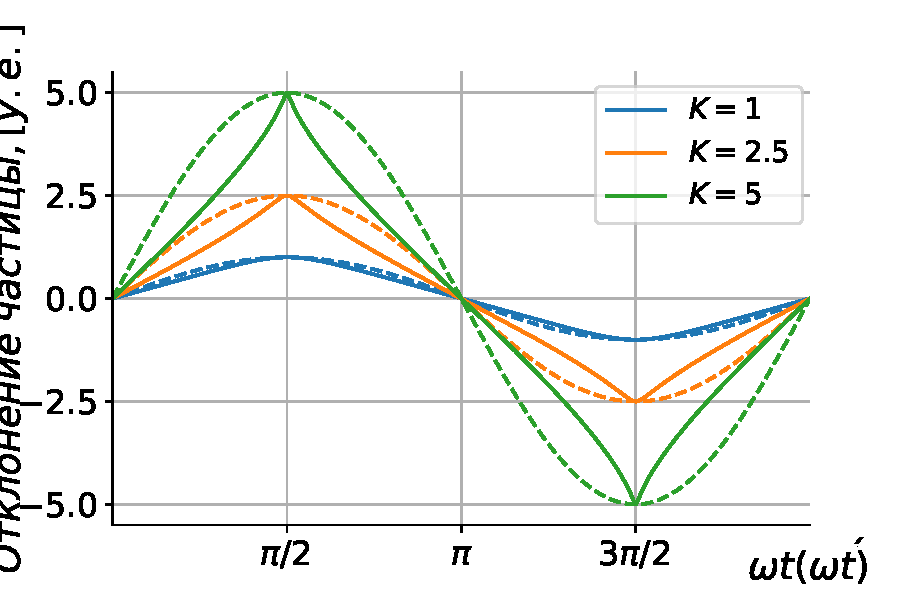
\includegraphics[width=\textwidth]{pic/emmiter_traj.pdf}
		\caption{Отклонение частицы при $\theta = 0$}
		\label{fig:emmiter_traj}
	\end{minipage}\hfill
	\begin{minipage}{0.49\textwidth}
		\centering
		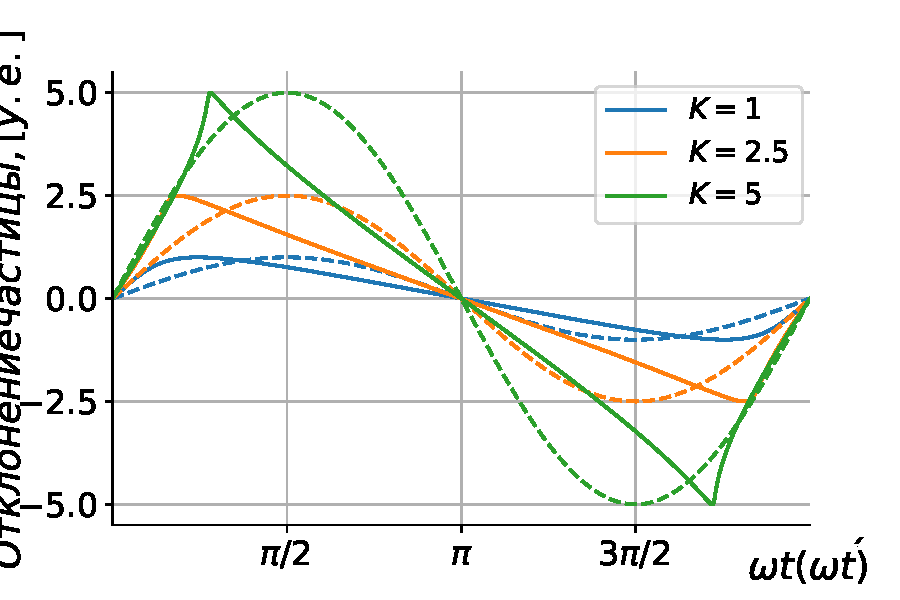
\includegraphics[width=\textwidth]{pic/emmiter_traj_ang.pdf}
		\caption{Отклонение частицы при $\theta = 1/\gamma$}
		\label{fig:emmiter_traj_ang}
	\end{minipage}    
\end{figure}
На рис.~\ref{fig:emmiter_traj} изображено отклонение частицы, видно, что наблюдатель видит искажённую траекторию, но при этом кривая обладает некоторой симметрией, а именно, при разложении в ряд Фурье мы получим слагаемые содержащие только нечётные гармоники: $\omega, 3\omega, 5\omega$ и т.д., чётные гармоники внесут ассимметрию, отсюда, излучение на оси всегда будет содрежать только нечётные гармоники. Но уже как видно из рис.~\ref{fig:emmiter_traj_ang}, при наблюдении по углом, траектрория становиться ассиметричной, разложение в ряд Фурье будет содержать слагаемые с $2\omega, 4\omega, 6\omega$ и т.д., в спектре появятся чётные гармоники.
\fi

\iffalse
\chapter{Элементы фурье оптики}
В этой главе мы предложим наглядный подход к решению задачи о распространение волнового фронта в пустом пространстве, его прохождении через систему линзу. Приведённые результаты напрямую могут быть использованы в программном коде. Распределение поля в начальный момент времени будем считать гауссовским, однако, как будет видно из изложения, подход может быть использован для произвольного распределения поля. В наших выкладкам мы в полной мере следуем подходу \cite{serkez2013grating} и \cite{serkez2015design}, полное изложение фурье оптики и статистической оптики можно найти в замечательных книгах \cite{goodman2015statistical}, \cite{goodman2005introduction}. В конце главы будет приведёт пример учебного кода \cite{my_github} для распространения волнового фронта через оптическую систему, написанный автором в рамках одного из университетских курсов.

\section{Распространение света в пустом пространстве}
Наши рассуждения мы начнём с волнового уравнения в пустом пространстве, т.е. $\vec{j} = 0, \rho = 0$. 
\begin{equation}
\pdv[2]{\vec{E}}{t} + c^2 \nabla^2 \vec{E} = 0
\end{equation}
В  $r\omega$-пространстве уравнение приобретает знакомый вид уравнения Гельмгольца, где $k_0 = \omega/c$.

\begin{equation}
k_0^2\vec{\widetilde{E}} + \nabla^2 \vec{\widetilde{E}} = 0
\end{equation}
Совершив фурье-преобразование в $k$-пространство по координатам $x,y$, которое определим схожим образом с~\ref{eq:Fourier_wt}:

\begin{equation}
\label{eq:Fourier_rk}
\begin{array}{lcl}
\vec{\widehat{E}}(\vec{k}, \omega) = \displaystyle\int\limits_{-\infty}^{\infty}\int\limits_{-\infty}^{\infty} dxdy \vec{E}(\vec{r}, t)\exp[ik_xx + ik_xx]\\
\\
\vec{E}(\vec{r}, \omega) = \cfrac{1}{4\pi^2}\displaystyle\int\limits_{-\infty}^{\infty}\int\limits_{-\infty}^{\infty} dk_xdk_y \vec{\widehat{E}}(\vec{k}, t)\exp[-ik_xx - ik_xx],
\end{array}
\end{equation}
получим: 
\begin{equation}
k_0^2\Big(1 - \cfrac{k^2_x}{k^2_0} - \cfrac{k^2_y}{k^2_0} \Big)\vec{\widehat{E}} + \dv[2]{\vec{\widehat{E}}}{z} = 0
\end{equation}
Теперь можно напрямую можно получить решение этого обыкновенного дифференциального уравнения:
\begin{equation}
\label{eq:sol}
\vec{\widehat{E}}(\omega, k_x, k_y, z) = \vec{\widehat{E}}(\omega, k_x, k_y, 0)\exp[ik_0z\sqrt{1 - \frac{k^2_x}{k^2_0} - \frac{k^2_y}{k^2_0}} ]
\end{equation}
На основе уравнения~\ref{eq:sol} введём функцию отклика среды:

\begin{equation}
\begin{array}{lcl}
H(k_x, k_y, z) = \cfrac{\vec{\widehat{E}}(\omega, k_x, k_y, z)}{\vec{\widehat{E}}(\omega, k_x, k_y, 0)} = \exp[ik_0z\sqrt{1 - \cfrac{k^2_x}{k^2_0} - \cfrac{k^2_y}{k^2_0}} ]
\\
\\
H(k_x, k_y, z) \approxeq \exp[k_0z]\exp[-\cfrac{iz}{2k_0}(k^2_x + k^2_y)]
\end{array}
\end{equation}
Видно, чтобы получить распределение электромагнитного поля на некотором расстоянии $z$, необходимо совершить обратное преобразование Фурье в $xy$-пространство. Таким образом решение волнового уравнения сводиться к трём относительно простым операциям: первое, --- перевод начального распределения в $k_xk_y$-пространство, далее домножение получившегося распределения на функцию отклика среды, в нашем случае пустое пространство, и последний шаг, --- обратное преобразование Фурье. Из вывода видно,что мы не накладывали никаких ограничений на начальное распределение поля, кроме, быть может, естественных ограничений, накладываемых на оригинал преобразованием Фурье.

\section{Действие тонкой линзы на волновой фронт}
В этом параграфе мы построим элементарную оптическую систему, состоящую из пустого промежутка, --- $d_1$, тонкой линзы с оптической силой, --- $1/f$ и ещё одного пустого промежутка до плоскости изображения. Действие тонкой линзы мы представим как домножение комплексной амплитуды поля на следующее выражение: 
\begin{equation}
T_f(x, y) = \exp[-\cfrac{ik_0}{2f}(x^2 + y^2)]
\end{equation}
Для предметности обсуждения определим начальное распределение гауссовым пучком: 

\begin{equation}
\overline{E}(x, y, 0) = A\exp[-\cfrac{x^2 + y^2}{w^2_0}]
\end{equation}
После преобразование Фурье в $k_xk_y$-пространстве мы получим:

\begin{equation}
\hat{E}(k_x, k_y, 0) = A\pi w^2_0\exp[-\cfrac{w^2_0}{4}(k_x^2 + k_y^2)]
\end{equation}
После домножения этого распределения поля в $k_xk_y$-пространстве на функцию отклика пустого промежутка, получим
\begin{equation}
\label{eq:after_lens}
\begin{array}{lcl}
\hat{E}(k_x, k_y, z) = \hat{E}(k_x, k_y, z)H(k_x, k_y, z) 
\\
\\
= A\pi w^2_0\exp[-\cfrac{w^2_0}{4}(k_x^2 + k_y^2)]\exp[k_0z]\exp[-\cfrac{iz}{2k_0}(k^2_x + k^2_y)]
\\
\\
= A\pi w^2_0\exp[k_0z]\exp[-\cfrac{iq}{2k_0}(k^2_x + k^2_y)], 
\end{array}
\end{equation}
здесь мы ввели $q = z - iz_R$, где $z_R = \cfrac{k_0w^2_0}{2}$. После перехода обратно в $xy$-пространство, получим: 
\begin{equation}
\overline{E}(x, y, z) = \cfrac{iAk_0w^2_0}{2q}\exp[k_0z]\exp[-i\cfrac{k_0}{2q}(x^2 + y^2)],
\end{equation}
Теперь можно воспользоваться выражением для тонкой линзы и получить:
\begin{equation}
\begin{array}{lcl}
\overline{E}_{l}(x, y, z) = T_f(x, y)\overline{E}(x, y, z) = 
\\
\\
\cfrac{iAk_0w^2_0}{2q}\exp[k_0z]\exp[-i\cfrac{k_0}{2q}(x^2 + y^2)]\exp[-\cfrac{ik_0}{2f}(x^2 + y^2)]
\\
\\
\cfrac{iAk_0w^2_0}{2q}\exp[k_0z]\exp[-i\cfrac{k_0}{2q_l}(x^2 + y^2)],
\end{array}
\end{equation}
где $\cfrac{1}{q_l} = \cfrac{1}{q} \; - \; \cfrac{1}{f}$. \\

Теперь можно подвести итог: после распространения волнового фронта на расстояние $d_1$ параметр $q$ преобразуется:
\begin{equation}
q(d_1) = q(0) + d_1, 
\end{equation}
далее на него действует линза: 
\begin{equation}
\cfrac{1}{q_l} = \cfrac{1}{q(0) + d_1} - \cfrac{1}{f},
\end{equation}
и ещё один пустой промежуток, до места, где волновой фронт опять будет плоским: 
\begin{equation}
q(d_1 + d_2) = q_l + d_2, 
\end{equation}
Условие того, что волновой фронт плоский мы сформулируем так, что $q(d_1 + d_2) = -i\cfrac{k_0w^2_2}{2}$, что легко проверятся подстановкой в~\ref{eq:after_lens}. Получим уравнение: 
\begin{equation}
-i\cfrac{k_0w^2_2}{2} = q_l + d_2, 
\end{equation}
где, приравниванием мнимых частей, получим: 
\begin{equation}
w^2_2 = \cfrac{f^2w^2_1}{(f - d_1)^2 + (k_0w^2_1/2)^2}
\end{equation}
то же для реальных частей: 
\begin{equation}
d_2 = f + f^2\cfrac{(d_1 - f)}{(d_1 - f)^2 + (k_0w^2_1/2)^2}
\end{equation}
Из последнего уравнения видно, что если положить перетяжку гауссового пучка раной нулю, то выражение переходит в соотношение геометрической оптики.

В приведённой главе мы дали краткий путь того, как можно очень эффективно и относительно просто использовать Фурье оптику для написания симуляционных кодов при проектировании оптических систем. В качестве примера, для заинтересованных читателей на веб-странице (веб-страница) приведёт код простой оптической системы, который в полной мере используют результаты вышеприведённого параграфа. Код был написан автором данной рукописи рамках курса <<Основы вычислительной физики>>, который читается на физическом факультете НГУ. Дальнейшие комментарии к коду можно найти в репозитории указанной по ссылке.
\fi

\chapter{Краткий обзор дифракции на кристаллах}
Основные кристаллы используемы на источниках синхротронного излучения --- это $Si$ (кремний), $C$ (алмаз) и реже $Ge$ (германий). Виду кубической кристаллической решётки эти кристаллы относительно просты при рассмотрение динамики отражение и преломления на кристаллических плоскостях. Для нас важны такие свойства кристаллов, как способность преобразовать относительно широкой спектр ондуляторного излучения $\Delta E/ E \sim 10^{-2}$ в излучение с относительной монохроматичностью до $\Delta E/ E \sim 10^{-4}$. 
\section{Симметричное брэгговское отражение от идеально кристалла}\label{diamond cry absorb}
Длины волн, которые отвечают резонансу при отражении падающего под углом $\theta$ к плоскости кристалла излучения, даётся законом Брэгга:  
%пропорциональный $\gamma / nN$, где $n$ --- номер гармоники излучения, $N$ --- число периодов ондулятора, а $\gamma$ --- гамма фактор релятивистского электрона
\begin{equation}
	m\lambda = 2d\sin\theta,
\end{equation}
где $d$ --- расстояние между плоскостями от которых происходит отражение, $m$ --- некоторое положительно целое число. Однако динамическая и кинематическая теории дифракции уточнаю данные результат и вносят конечную угловую и/или энергии ширину, в которую кристалл может принять излучение, а также некоторый сдвиг, относительно предполагаемого брэгговского угла. Кривая, которая описывает отражательную способность кристалла, называется кривой Дарвина, именно она определяет, в нашем случае, угловой акцептанс кристалла. На рис.~\ref{fig:bragg_R} показаны характерные кривые отражение для алмаза и кремния. 
\begin{figure}
	\centering  
	\begin{minipage}{0.49\textwidth}
		\centering
		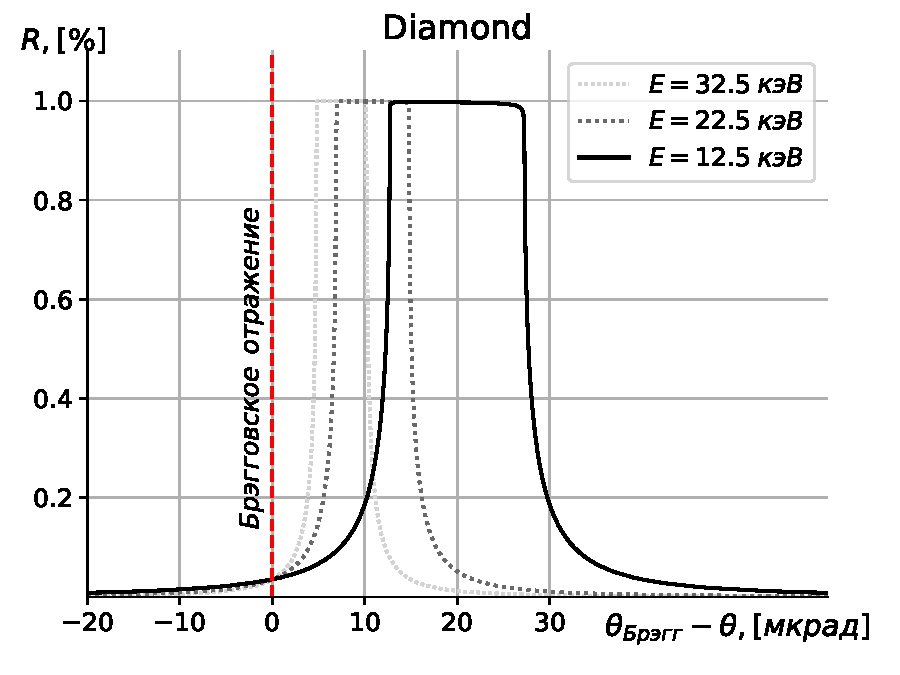
\includegraphics[width=\textwidth]{pic/Diamond_bragg_R.pdf}
		\caption{Кривая Брегга для алмаза на разных энергиях падающего излучения}
		\label{fig:bragg_R}
	\end{minipage}\hfill
	\begin{minipage}{0.49\textwidth}
		\centering
		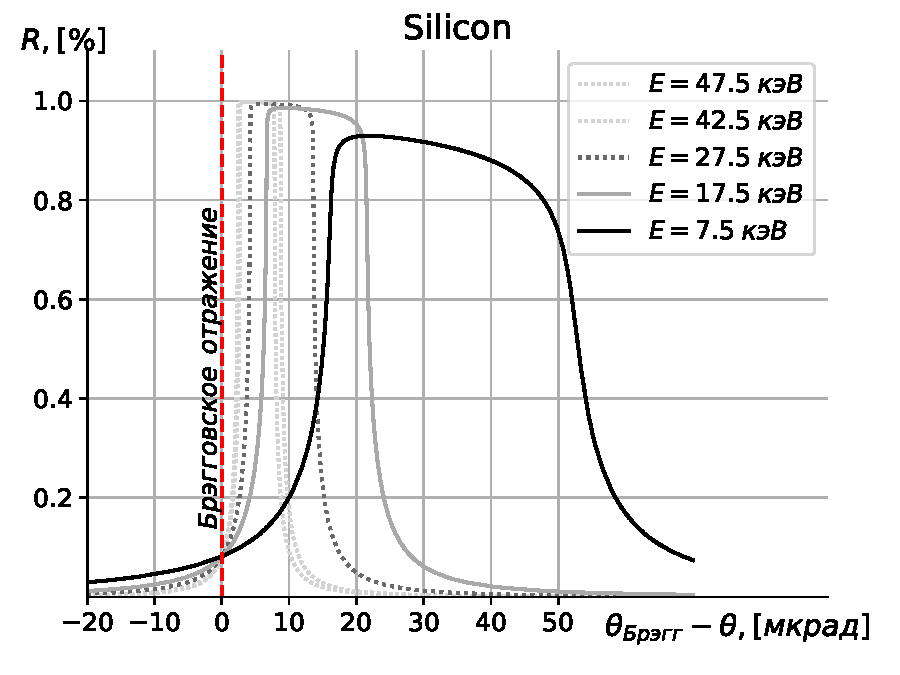
\includegraphics[width=\textwidth]{pic/Silicon_bragg_R.pdf}
		\caption{Кривая Брегга для кремния на разных энергиях падающего излучения}
		\label{fig:bragg_T}
	\end{minipage}    
\end{figure}
При расчёте кристаллов монохроматоров характер кривой Дарвина необходимо учитывать, чтобы доставить эффективную работу кристалла и уменьшить тепловые нагрузки: угловая расходимость излучения должна входить в акцептанс кристалла, иначе излучение поглотится в кристалле. 

В целом, данной информации достаточно, чтобы иметь первое представление необходимое для разработки оптических трактов синхротронного излучения. Для дальнейшего чтения и углубления знаний в данном вопросе могут быть полезны следующие книги \cite{als2011elements}, \cite{authier2006dynamical}.

%\section{Поглощательные способности кристаллов}
%Одним из полезных применений кристаллов в рентгеновском диапазоне есть их фильтрующая способность, отрезать низкие энергии, в особенности для алмазных кристаллов, которые, по мимо всего, имеют хорошую теплопроводность, что способствуют быстрому теплоотводу. На рис.~\ref{fig:bragg_T} представлена кривая поглощения 100 мкм кристалла алмаза. Подобные кристаллы устанавливают перед первыми оптическими элементами, что в значительной степени снижает тепловые нагрузки, подавляя низшие гармоники, в нашем случае ондуляторного излучения. 

\chapter{Дополнительные графики} \label{AppendixA}
\begin{figure}[h!]
	\centering  
	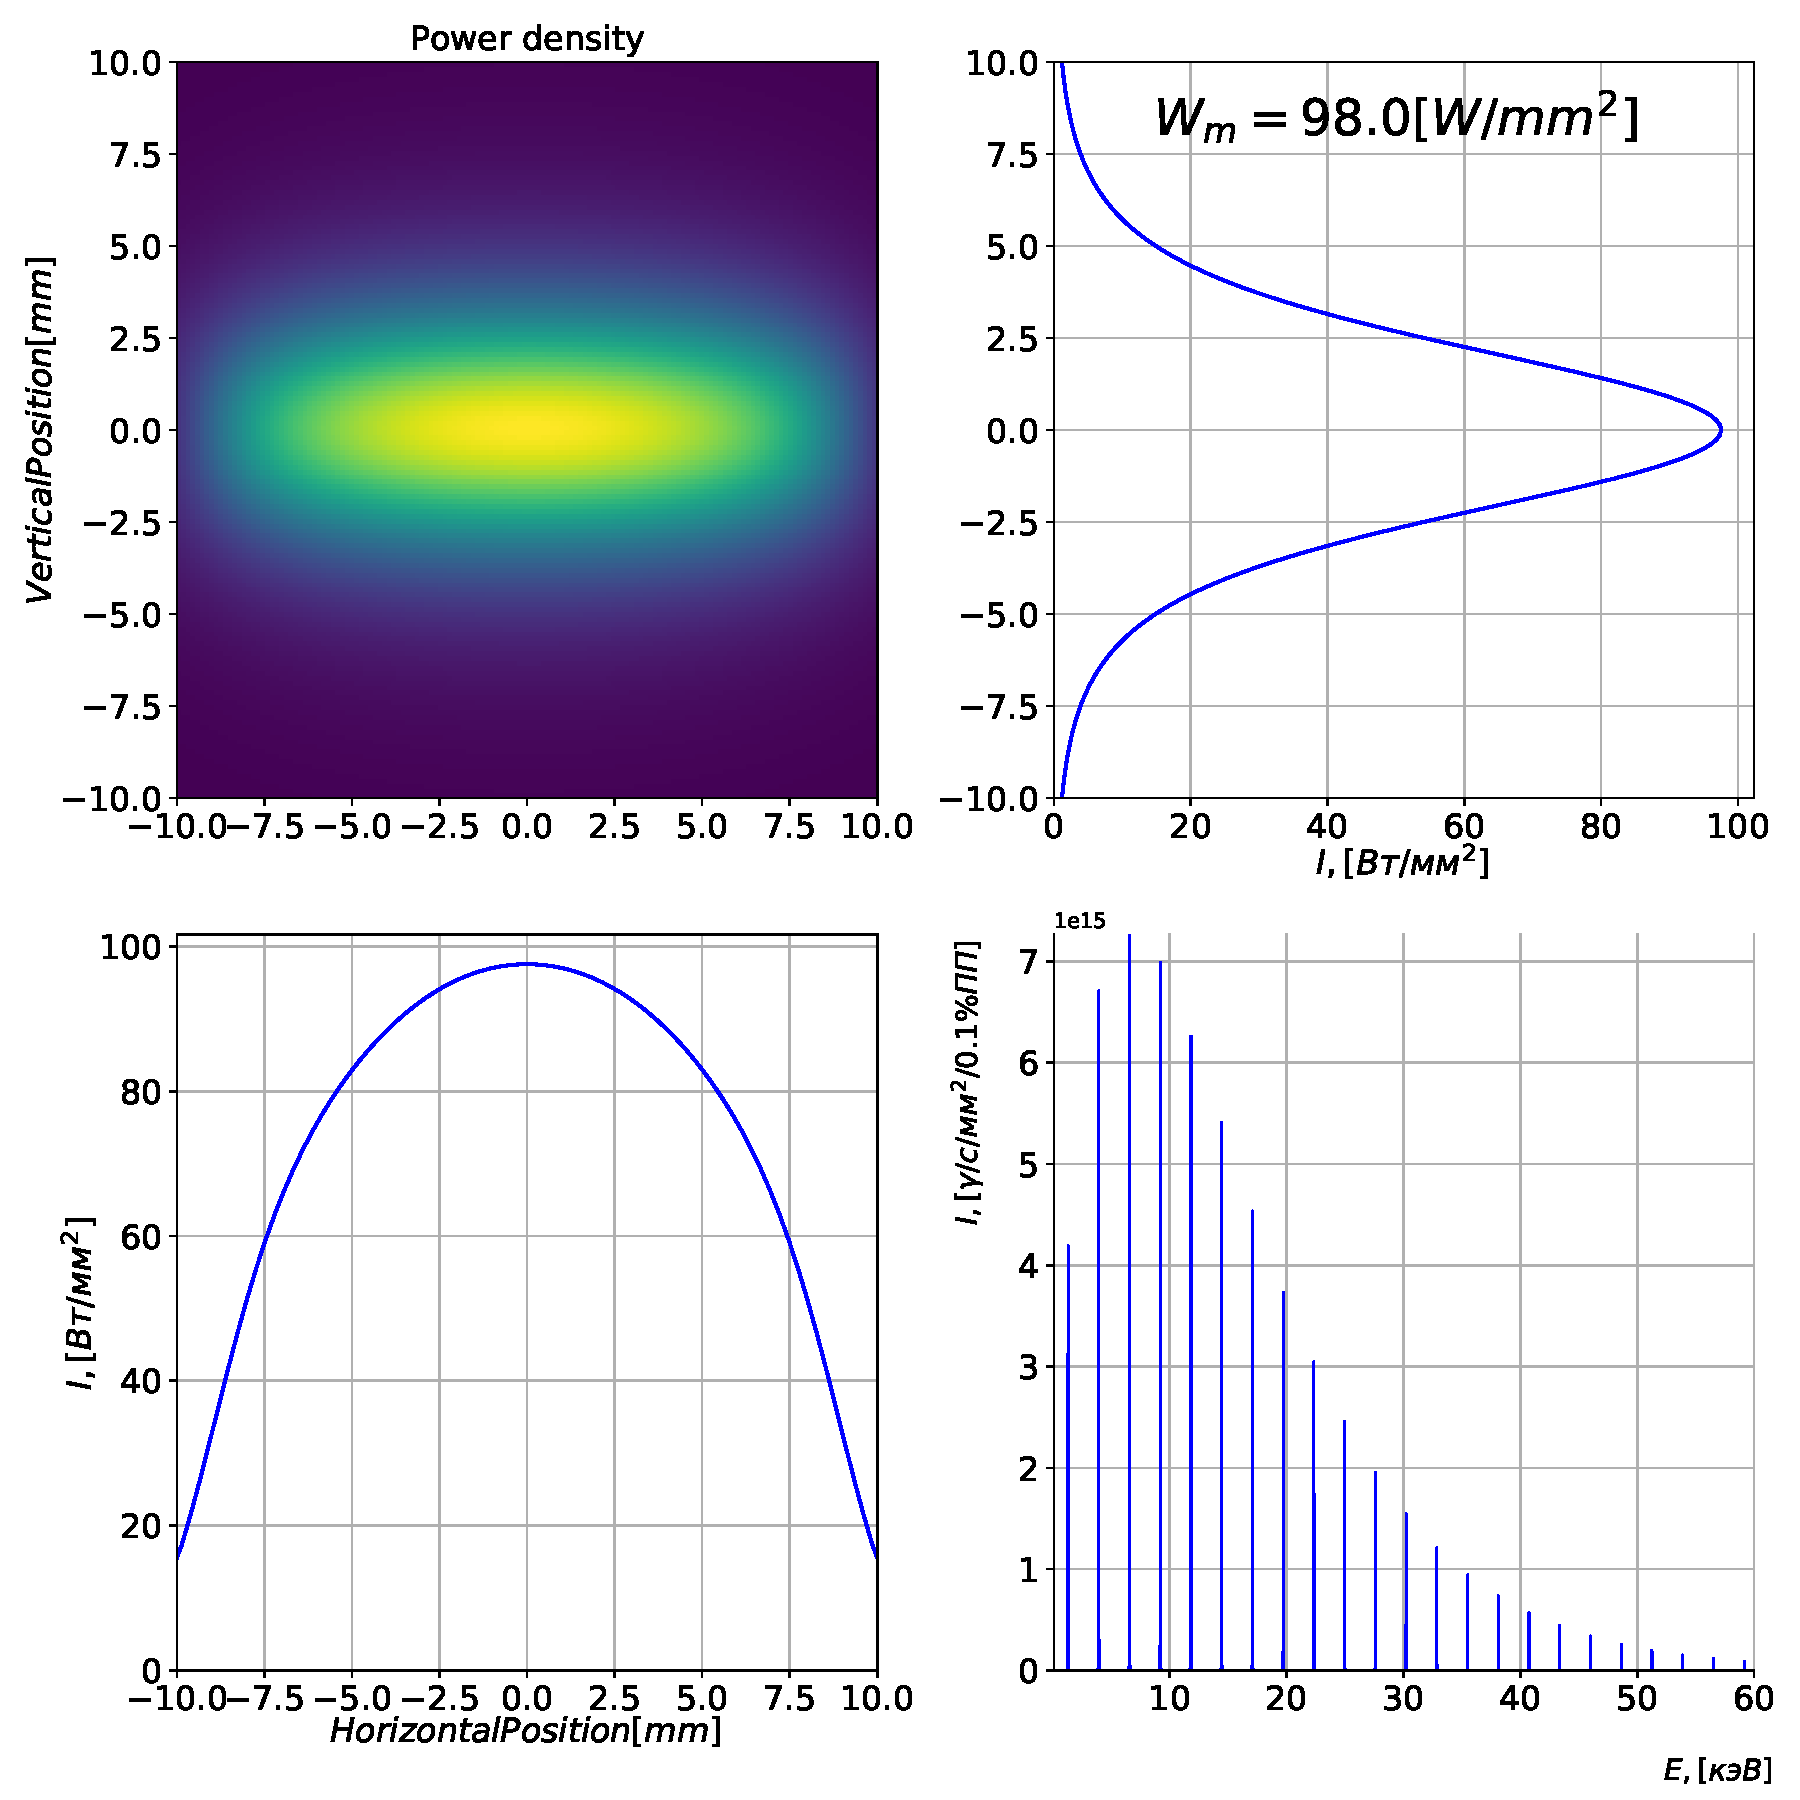
\includegraphics[width=\textwidth]{pic/power_dens_1-1.pdf}
	\caption{Плотность мощности для используемого ондулятора и его срезы на оси $x$ и $y$ через точку максимума распределения и спектр уединённого электрона (правый нижний)}
	\label{fig:power_dens_1-1}  
\end{figure}
\begin{figure}[h!]
	\centering  
	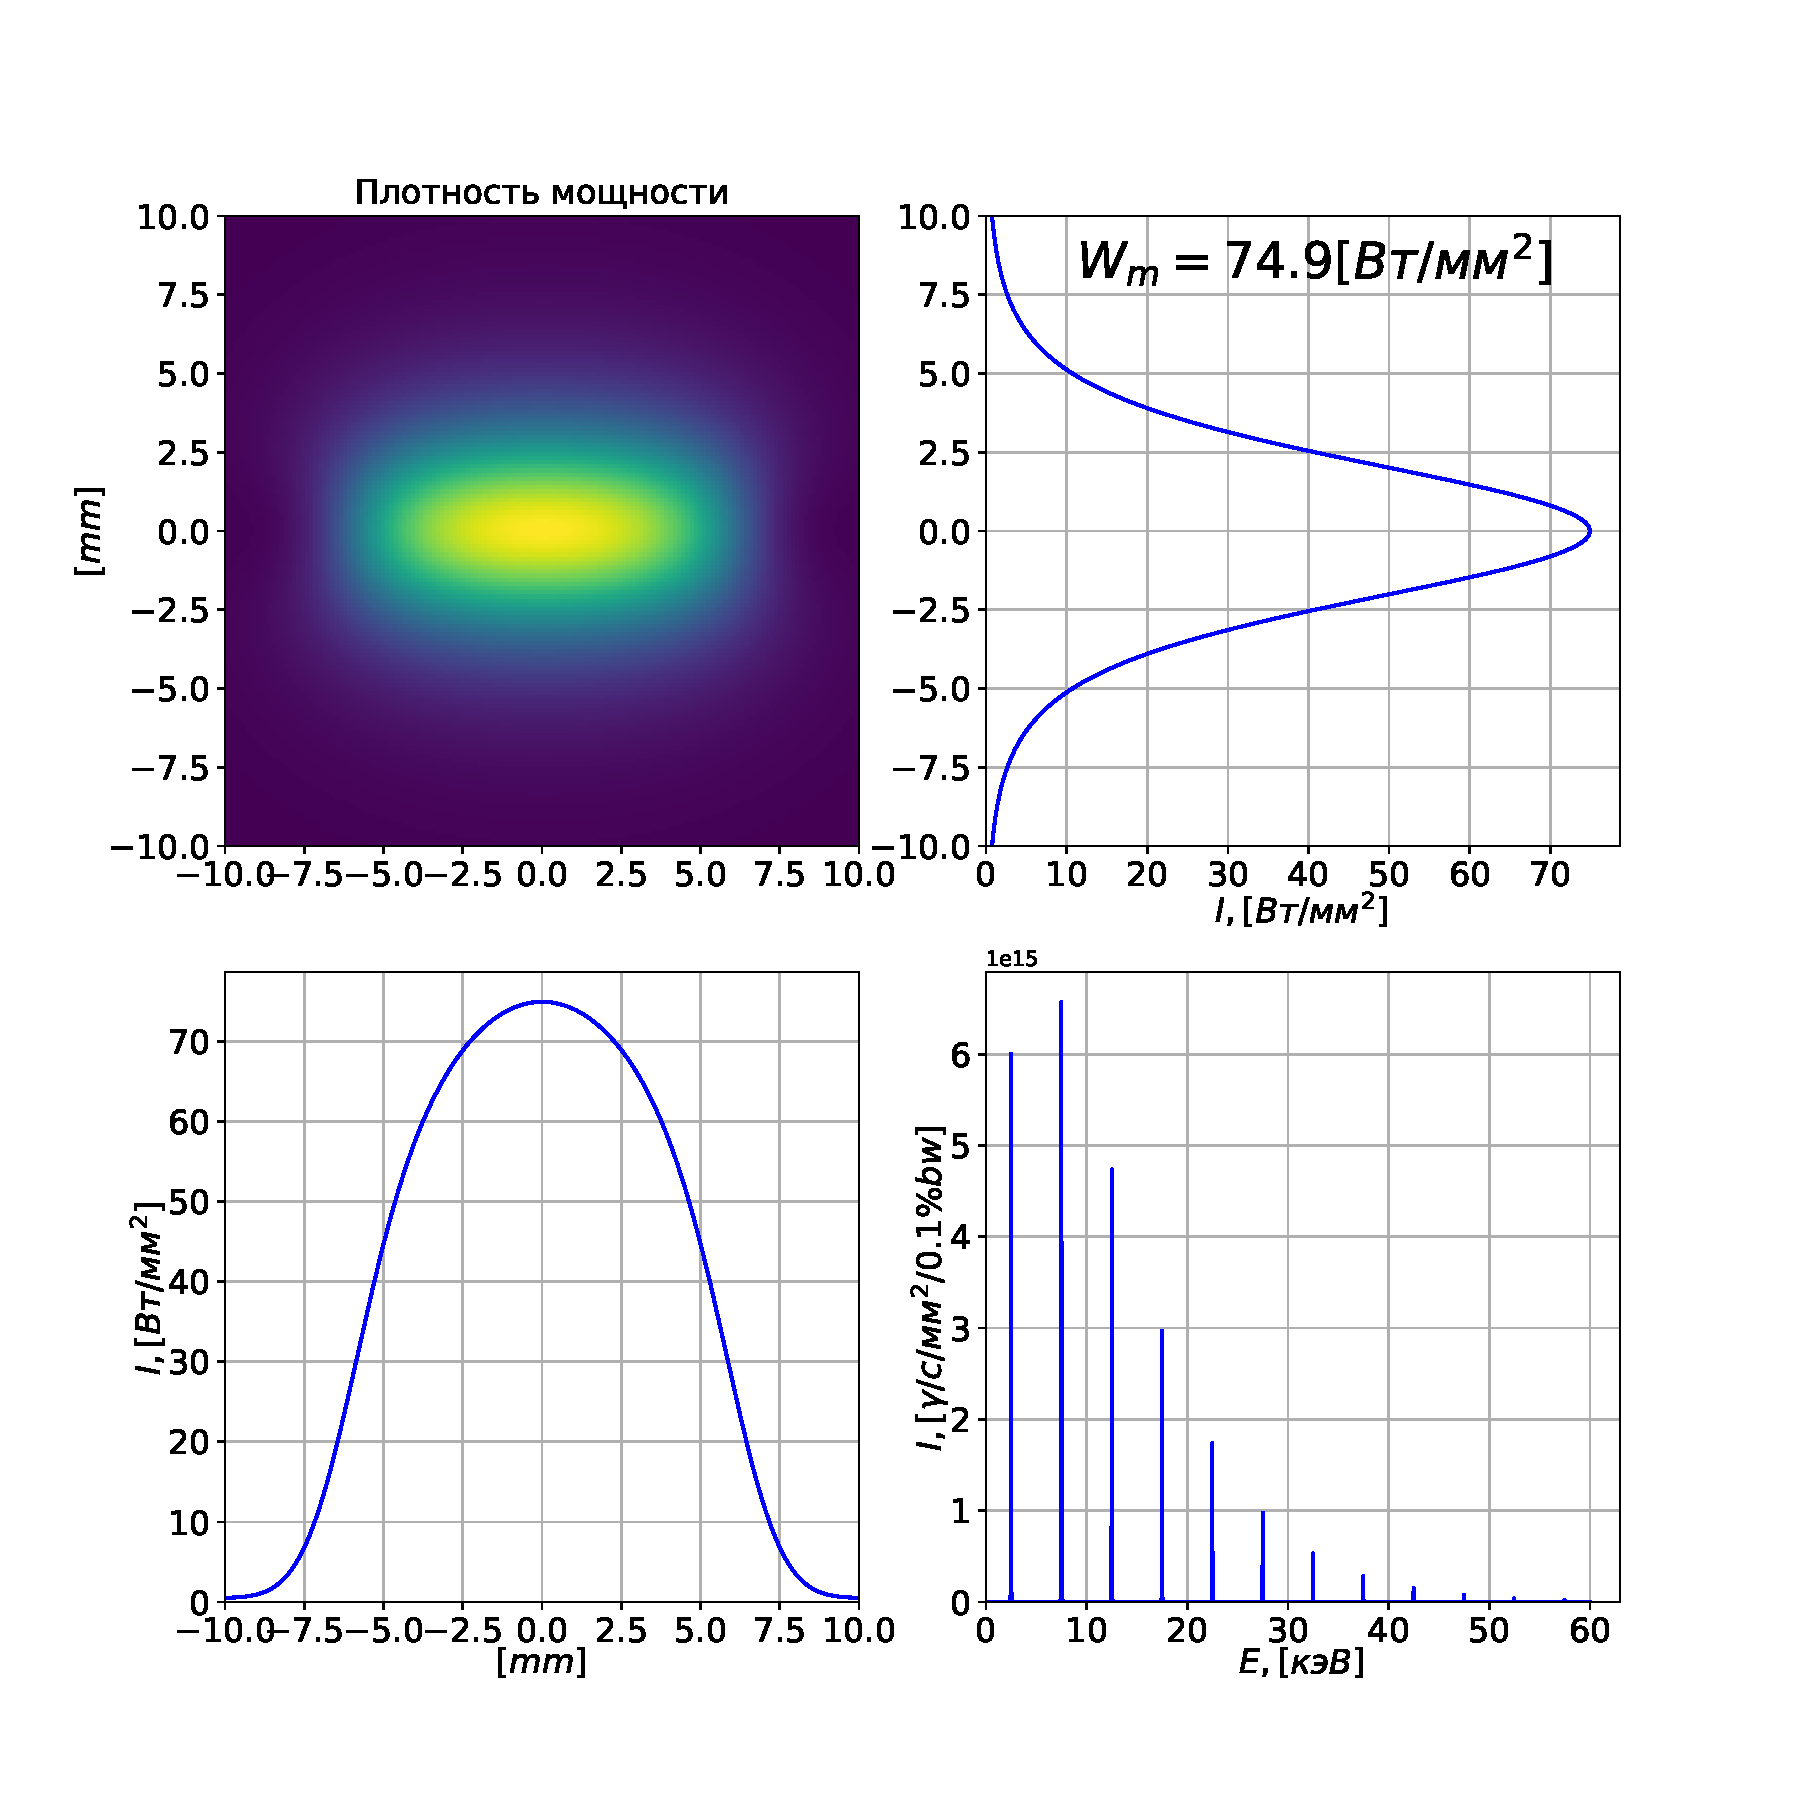
\includegraphics[width=\textwidth]{pic/power_dens_1-2.pdf}
	\caption{Плотность мощности для используемого ондулятора и его срезы на оси $x$ и $y$ через точку максимума распределения и спектр уединённого электрона (правый нижний)}
	\label{fig:power_dens_1-2}   
\end{figure}
\begin{figure}[h!]
	\centering  
	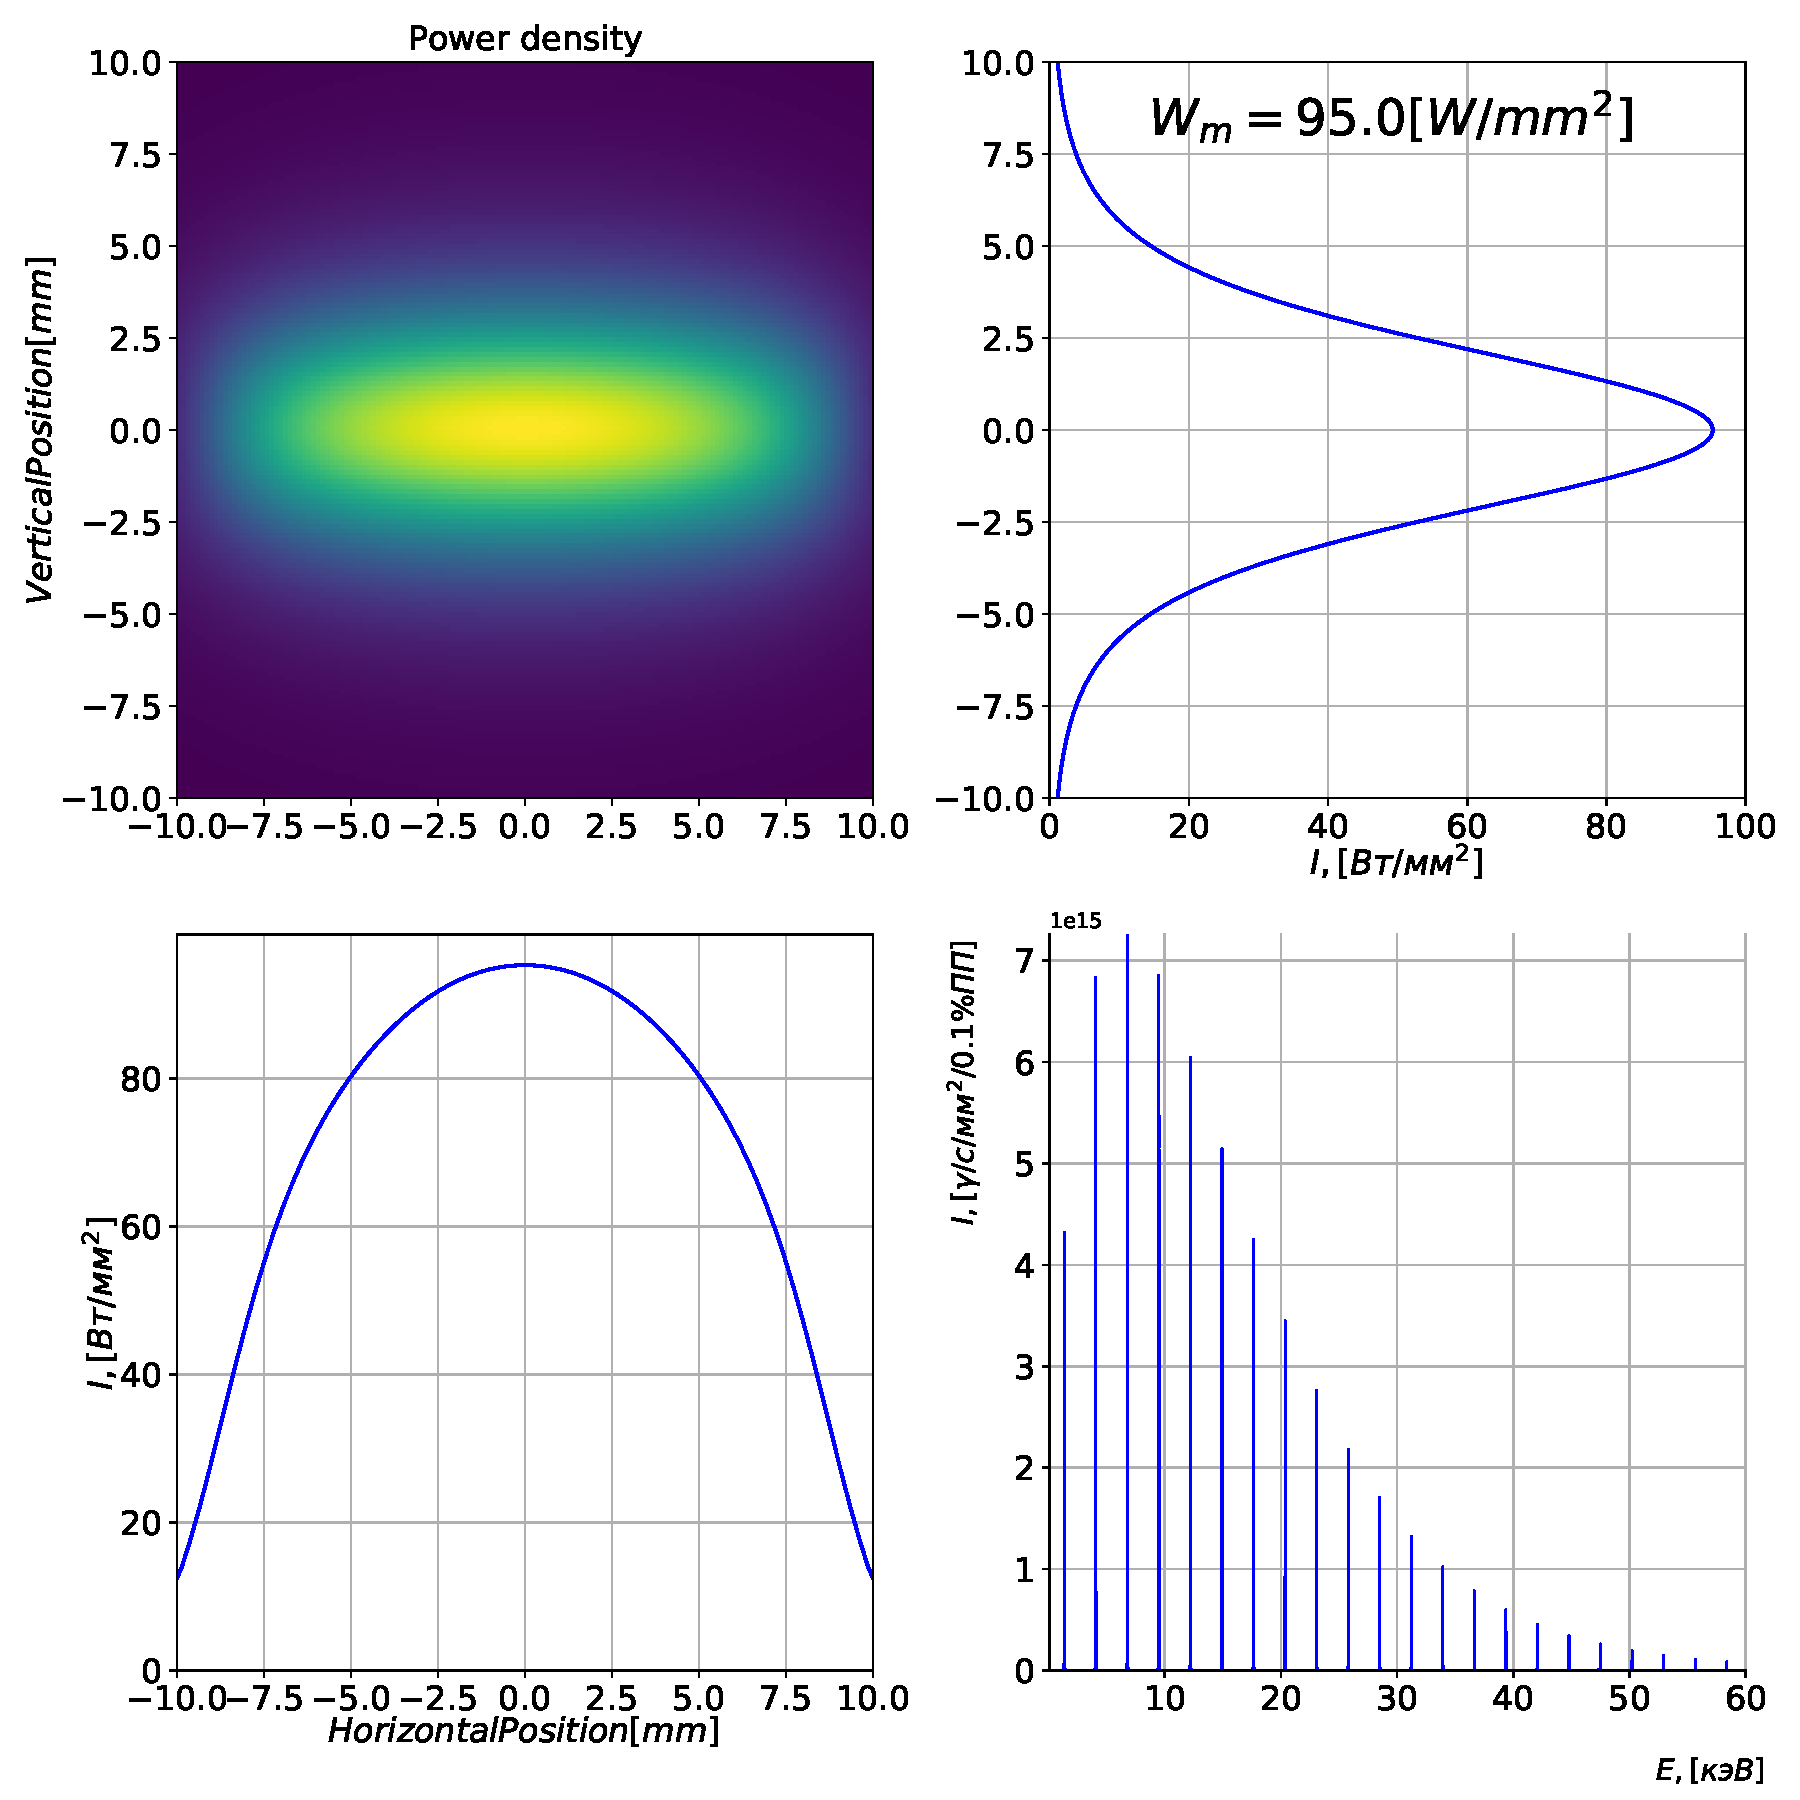
\includegraphics[width=\textwidth]{pic/power_dens_1-4.pdf}
	\caption{Плотность мощности для используемого ондулятора и его срезы на оси $x$ и $y$ через точку максимума распределения и спектр уединённого электрона (правый нижний)}
	\label{fig:power_dens_1-4}   
\end{figure}

\chapter{Примеры программного кода} \label{AppendixB}

\section{Подраздел приложения}\label{AppendixB1}

\normalsize% возвращаем шрифт к нормальному
